\chapter{微生物组与共生}\label{ch:b3:microbiomes}

你体内约携带 38 万亿个细菌，大致与你自身的细胞数相当，
其中大多数位于肠道末端的最后一米，
它们的重量约与你的大脑相当，携带的基因
数量是你的一百倍。无菌饲养的小鼠
为维持体重需多吃约三分之一的食物，免疫系统发育不良，
行为也颇为异常。豌豆植株把其糖分的十分之一供给根部\omterm{def:b3:microbiomes:nodule}{根瘤}中的细菌，
并以此换取氮素；全部陆生植物中有五分之四，
与包绕根系的真菌以糖换磷，
这种\omterm{def:b3:microbiomes:symbiosis}{共生}已持续四亿年；珊瑚是一种动物，
在细胞内饲养藻类，海水变暖到足以使其
驱逐它们时便会死亡。生物并非孤立的个体，而是联合体，并
本章讨论伙伴关系的生物学：它们如何
借助测序进行计数与刻画，伙伴之间交换什么，
这种交换如何协商与监管，以及为何某些伙伴
最终演化为细胞器。

\section{共生相关术语}

\begin{definition}[共生]\label{def:b3:microbiomes:symbiosis}
\index{共生}\index{互利共生}\index{偏利共生}\index{共生功能体}\index{微生物组}\index{垂直传播}
\emph{共生}是指不同物种的生物体之间持续而紧密的联系，
两者皆获益时为\emph{互利共生}，
一方获益而另一方不受影响时为\emph{偏利共生}，
一方获益而另一方受损时为寄生——同一对伙伴可以
随条件沿此连续谱移动。\emph{内共生体}
生活在宿主细胞内；\emph{专性}伙伴不能
单独生存。共生体\emph{垂直地}传递，即从亲代传给子代
（蚜虫的 \emph{Buchnera} 经卵传递），或
\emph{水平地}传递，每代都从环境中重新获得，
或从其他宿主处获得（乌贼的 \emph{Vibrio}、人类肠道细菌）。
\emph{微生物组}是某一生境中全部微生物的群落，
如肠道、叶表面、一克土壤——而
\emph{共生功能体}是宿主连同其微生物组，
被视为自然选择作用的单位。
\end{definition}

\begin{example}[三种专性伙伴]\label{ex:b3:microbiomes:obligate}
蚜虫体内的 \emph{Buchnera} 已在宿主细胞内生存了两
亿年，能合成韧皮部汁液所缺乏的必需氨基酸，
并将基因组压缩至\qty{640}{kb}，仅为其
自由生活近缘种的七分之一——丢失了宿主现已提供的每一个基因。
细菌 \emph{Wolbachia} 存在于三分之二的昆虫物种中，
仅经卵传递，因而演化为偏向雌性：它
令雄性胚胎死亡、使其雌性化，或使未感染雌性的卵
在被感染雄性受精时死亡（\emph{细胞质
不亲和}），从而在种群中扩散。携带它的蚊子
传播登革热的能力较弱，释放它们已使
若干城市的登革热明显下降。变形虫 \emph{Paulinella} 曾
在约一亿年前吞入一种蓝细菌，它如今既非
完全的细菌，也非完整的叶绿体——
是光合细胞器的第二次独立起源，恰好停在中途。
\end{example}

\section{群落的计数}

\begin{method}[通过测序分析微生物组]\label{met:b3:microbiomes:16s}
\index{16S rRNA 测序}\index{宏基因组学}\index{操作分类单元}
多数微生物无法培养，因而通过其 DNA 进行计数。（1）
提取样品中的 DNA——粪便、土壤，或过滤到
滤膜上的海水。（2）一是扩增小亚基核糖体
RNA 基因（\emph{16S}），\omterm{def:b3:genetic-engineering:pcr}{引物}与其通用区匹配，并
对其间的可变区测序——这是一种\emph{扩增子}调查，
成本低廉，能将细菌鉴定到大致属的水平，
并按读段数计数；或对全部 DNA 测序——\emph{鸟枪法
\omterm{met:b3:microbiomes:16s}{宏基因组学}}，可获得基因乃至整个基因组，
因而能说明群落的功能潜力，而不仅是其中有哪些成员。（3）将读段
聚类为序列变体或\emph{\omterm{met:b3:microbiomes:16s}{操作分类单元}}（OTUs，
通常以 \qty{97}{\%} 相似度界定一个“物种”），并
将其与数据库\omterm{def:b3:bioinformatics:alignment}{比对}进行归类（见\cref{ch:b3:bioinformatics}），
并按样品制表统计计数。（4）计算样品内的多样性，
比较样品间的组成。计数是相对的——
一个样品的读段总数固定——且会因提取、
\omterm{def:b3:genetic-engineering:pcr}{引物}和拷贝数而产生偏差，因此以相同方式处理的
样品间差异可信，绝对数值则不然。
\end{method}

\begin{definition}[多样性]\label{def:b3:microbiomes:diversity}
\index{物种丰富度}\index{香农指数}\index{辛普森指数}\index{稀疏化}
设一个含 $S$ 个物种的群落，相对丰度分别为 $p_{1},\dots,
p_{S}$（$\sum p_{i} = 1$）：\emph{丰富度}为 $S$；
\emph{香农指数} $H = -\sum_{i} p_{i}\ln p_{i}$ 度量了
随机抽取一个个体时其物种归属的不确定度，而
$e^{H}$ 是能产生相同不确定度的等丰度物种数
（即有效物种数）；\emph{辛普森
指数} $D = \sum_{i} p_{i}^{2}$ 是随机抽取的两个个体属于同一物种的概率，
而 $1/D$ 是另一种有效物种数，
其权重偏向常见物种。丰富度取决于
所观察个体的数量：\emph{稀疏曲线}
以所发现的物种数对取样个体数作图，并
在大多数物种已被发现后趋于平缓。
\end{definition}

\begin{theorem}[稀疏化]\label{thm:b3:microbiomes:rarefaction}
\index{稀疏化!公式}\index{古德覆盖度}
一个样品含 $N$ 个个体、$S$ 个物种，物种个体数分别记为 $N_{i}$
（$i$ 为物种编号）。从样品中不放回地抽取一个含 $n$
个个体的随机子样本，其物种数的期望为
\[
E[S_{n}] = \sum_{i=1}^{S}\left[1 - \frac{\binom{N - N_{i}}{n}}
{\binom{N}{n}}\right],
\]
该期望随 $n$ 增大，以 $S$ 为上界，并在 $n = N$ 时取到。两个大小
不同的样品通过将二者\omterm{def:b3:microbiomes:diversity}{稀疏化}到相同的 $n$ 进行比较。群落中
属于尚未观察到的物种的个体所占比例
由\emph{\omterm{thm:b3:microbiomes:rarefaction}{古德覆盖度}}估计，约为 $f_{1}/N$，其中
$f_{1}$ 为只被观察到一次的物种数（即单例）。
\end{theorem}
\begin{proof}
物种 $i$ 不出现在子样本中，当且仅当全部 $n$
个个体均取自其余 $N - N_{i}$ 个个体，
这种情形在 $\binom{N - N_{i}}{n}$ 个（共 $\binom{N}{n}$ 个等可能子样本）中发生；
因此物种 $i$ 出现的概率为 $1 - \binom{N-N_{i}}{n}/
\binom{N}{n}$，因而出现的物种数期望等于
这些概率之和（示性变量和的期望）。每一项
随 $n$ 增大而增大，且在 $n = N$ 时，分子中每个二项式
均为零。古德估计：下一个抽到的个体属于未被发现的
物种的概率，约等于随机选取的样品个体
恰是其物种中唯一的一个，即 $f_{1}/N$（古德，1953）；
其论证在本阶段不加证明地承认。
\end{proof}

\begin{example}[两个肠道]\label{ex:b3:microbiomes:two-guts}
取自某人的 $1000$ 条读段样本得到 $150$ 个物种，其中
$H = 3.5$，单例数 $40$；另一人的 $5000$ 条读段样本
得到 $260$ 个物种。第二个样本未必多样性更高：它
的取样深度是前者的五倍，若将其\omterm{def:b3:microbiomes:diversity}{稀疏化}至 $1000$ 条读段，
也可能得到 $150$ 个物种。第一个样本的覆盖度为 $1 - 40/1000 =
\qty{96}{\%}$：该肠道中百分之四的细菌属于
样本从未见过的物种，更深的取样将会发现它们。
有效物种数 $e^{3.5} \approx 33$，相当于 33 个物种的均匀度，
而丰富度为 $150$，说明少数物种占据主导——
这正是每个肠道的常态。
\end{example}

\begin{omfigure}
\begin{tikzpicture}
\begin{axis}[
  width=0.68\linewidth, height=5.6cm,
  axis x line=bottom, axis y line=left,
  xmin=0, xmax=5000, ymin=0, ymax=300,
  xlabel={取样读段数，$n$}, ylabel={观察到的物种数},
  xlabel style={font=\small, at={(axis description cs:0.5,-0.12)}, anchor=north}, ylabel style={font=\small},
  tick label style={font=\small}, xtick={0,1000,2000,3000,4000,5000}, ytick={0,100,150,200,260},
  clip=false,
]
\addplot[very thick, omDef, domain=0:5000, samples=60] {260*(1-exp(-x/1500))};
\addplot[very thick, omThm, domain=0:1000, samples=30] {150*(1-exp(-x/300))*1.0};
\addplot[very thick, omThm, dashed, domain=1000:5000, samples=30] {150*(1-exp(-x/300))*1.0 + 8*(1-exp(-(x-1000)/2000))};
\draw[dashed, gray] (axis cs:1000,0) -- (axis cs:1000,300);
\node[font=\scriptsize, omDef, anchor=north west] at (axis cs:1200,292) {第二个肠道：$260$ 个物种，$5000$ 条读段};
\node[font=\scriptsize, omThm, anchor=north east] at (axis cs:4900,140) {第一个肠道：$150$ 个物种（$1000$ 条读段），接近平台期};
\node[font=\scriptsize, gray, anchor=south west] at (axis cs:1050,10) {在此处稀疏化以便比较};
\end{axis}
\end{tikzpicture}

{\small 稀疏曲线。观察到的物种数随取样读段数增加而上升，
并在群落被充分取样后趋于平缓；两个样本在
相同深度下比较。此处第二个肠道在 $5000$ 条读段时仍在上升，
故其真实丰富度更高。}
\end{omfigure}

\section{人体微生物组}

\begin{definition}[肠道群落]\label{def:b3:microbiomes:gut}
\index{肠道微生物组}\index{短链脂肪酸}\index{定植抗性}\index{菌群失调}
人体肠道约含 $4\times 10^{13}$ 个细菌，几乎全部位于
结肠，每克内容物含 $10^{11}$ 个，相比之下，每克内容物
在酸性的胃中为 $10^{3}$ 个，沿小肠为 $10^{4}$--$10^{7}$ 个，而小肠
内食物流动迅速、胆汁对细菌不利。每人通常有五百到一千
个物种，多数属于两个门，即拟杆菌门和
厚壁菌门，几乎全为厌氧菌；每人所含的菌种各不相同，且
多年保持稳定，主要在生命最初三年内经由
母亲和家庭获得并定型。其作用是：发酵人体酶无法消化的
膳食纤维，生成\emph{短链脂肪酸}——
乙酸盐、丙酸盐、丁酸盐，它们为结肠细胞自身提供营养，
并可为宿主提供至多十分之一的热量；合成维生素~K 及部分 B
族维生素；转化胆汁酸与药物；占据每一生态位，使入
侵者无立足之地（\emph{定植抗性}）；并训练
免疫系统，其中调节性 T~细胞与分泌 IgA 的细胞
在其刺激下发育（见\cref{ch:b3:adaptive-immunity}）。一个
偏离此状态的群落——物种减少、
发酵菌减少、兼性需氧菌增多——即为\emph{菌群失调}，见于
炎症性肠病、使用\omterm{def:b3:bacteriology:antibiotics}{抗生素}之后，以及肥胖，尽管
其中因果关系通常并不清楚。
\end{definition}

\begin{proof}[证据]
在无菌隔离器中饲养的无菌小鼠（戈登及其同事，
2000 年代）肠壁薄、淋巴器官小、抗体水平
低，并需多摄入 \qty{30}{\%} 的热量以维持体重；
若定植以正常小鼠的微生物群，两
周内即长出脂肪。若给予肥胖小鼠而非瘦小鼠的微生物群，
无菌小鼠在相同食物下积累了更多脂肪（特恩鲍，2006）：
群落本身影响能量获取。在人类中，反复发作的
\emph{Clostridioides difficile}结肠炎——一种\omterm{def:b3:microbiomes:gut}{菌群失调}，其中
\omterm{def:b3:bacteriology:antibiotics}{抗生素}已清除了产毒\omterm{def:b3:bacteriology:phases}{芽孢
形成}菌的竞争者——\qty{94}{\%} 的患者经输注
健康供体粪便而治愈，相比之下，标准\omterm{def:b3:bacteriology:antibiotics}{抗生素}为 \qty{31}{\%}，
（范努德，2013）：这是首个随机试验，其中
起作用的药物是一个群落，而非一种分子。
\end{proof}

\begin{omfigure}
\begin{tikzpicture}
\begin{axis}[
  width=0.68\linewidth, height=5.4cm,
  ybar, bar width=18pt,
  axis x line=bottom, axis y line=left,
  ymode=log, ymin=1, ymax=1e13,
  symbolic x coords={stomach, duodenum, jejunum, ileum, colon},
  xtick=data, xticklabels={胃, 十二指肠, 空肠, 回肠, 结肠}, ytick={1e1,1e3,1e5,1e7,1e9,1e11},
  ylabel={每克内容物中的细菌数},
  ylabel style={font=\small}, tick label style={font=\small},
  clip=false,
]
\addplot[fill=omDef!40, draw=omDef] coordinates {(stomach,1e3) (duodenum,1e4) (jejunum,1e5) (ileum,1e7) (colon,1e11)};
\node[font=\scriptsize, anchor=west, xshift=10pt] at (axis cs:stomach,3e3) {酸性，pH 2};
\node[font=\scriptsize, anchor=south] at (axis cs:jejunum,1.5e5) {胆汁，流速快};
\node[font=\scriptsize, anchor=south, align=center] at (axis cs:colon,1.5e11) {慢速、厌氧：\\发酵菌};
\end{axis}
\end{tikzpicture}

{\small 沿人体肠道的细菌密度，采用对数尺度：
自酸性的胃到结肠，细菌密度上升了约一亿倍，此处
几乎聚集了全身绝大部分的微生物。}
\end{omfigure}

\begin{omfigure}
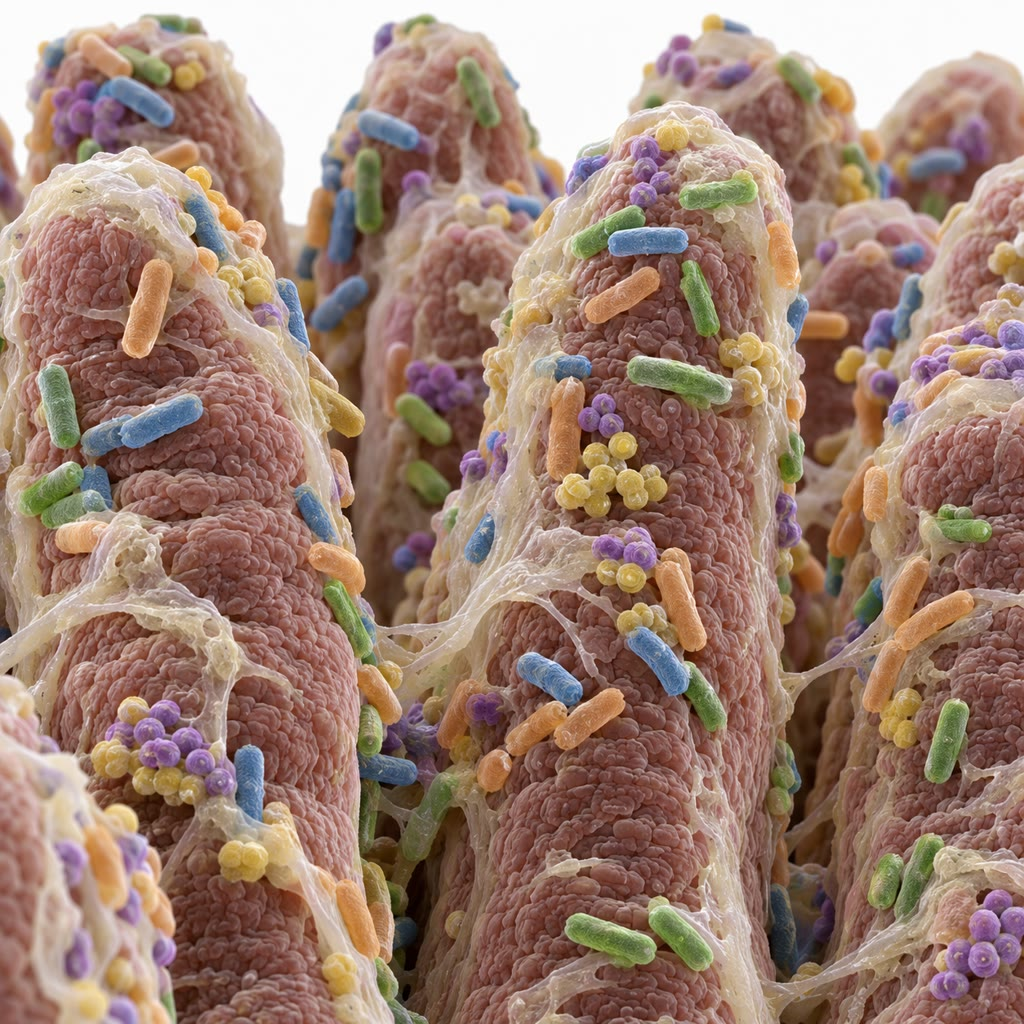
\includegraphics[width=0.40\linewidth]{images/book5/ai/b5-14-gut-microbiota.jpg}

{\small 肠黏膜表面在扫描电子
显微镜下的形貌，多种细菌滞留于
绒毛之间的黏液中。}
\end{omfigure}

\section{植物及其伙伴}

\begin{definition}[豆科植物与根瘤菌的共生]\label{def:b3:microbiomes:nodule}
\index{根瘤菌}\index{根瘤}\index{结瘤因子}\index{豆血红蛋白}\index{固氮酶}
豆科植物将固氮细菌（\emph{根瘤菌}）
容纳于\emph{根瘤}之中，根瘤是经分子层面的“对话”后专为此而建成的器官。
根分泌黄酮类物质；物种相符的根瘤菌
以\emph{结瘤因子}应答——它们是脂壳寡糖，其修饰基团
决定伙伴身份；根毛上的受体激酶与之结合，并
触发细胞核内钙离子振荡，并促使根毛
卷曲包住细菌，并形成\emph{侵染线}，它
穿过细胞向内生长，与此同时下方的皮层开始分裂，
形成根瘤。细菌被包在膜内释放进入根瘤细胞，
并分化为\emph{类菌体}，类菌体表达
\emph{固氮酶}，即将 N$_{2}$ 还原为氨的酶，
每分子消耗十六个 ATP。固氮酶受氧破坏，
但类菌体呼吸旺盛，根瘤以此化解这一矛盾，
借助扩散屏障和\emph{豆血红蛋白}，
一种植物血红蛋白，它紧密结合氧并将其运送至类菌体，
使游离氧维持在较低浓度——切开的根瘤之所以呈粉红色，正源于此。
植物为此付出其光合产物的百分之六至十，
并获得其大部分氮素；全球豆科作物所固定的氮，
已接近化肥工业的固氮量。
\end{definition}

\begin{omfigure}
\begin{tikzpicture}[every node/.style={font=\scriptsize}, >=stealth]
  % stage 1: root hair and bacteria, flavonoid / Nod factor exchange
  \begin{scope}
    \draw[thick, omMeth!60!black, fill=omMeth!15] (0,0) rectangle (1.2,3.0);
    \draw[thick, omMeth!60!black, fill=omMeth!15] (1.2,1.6) .. controls (2.4,1.7) and (2.6,2.6) .. (2.9,2.4) .. controls (2.5,2.3) and (2.3,1.4) .. (1.2,1.2) -- cycle;
    \foreach \p in {(3.1,2.7),(3.4,2.3),(3.3,1.9)} \fill[omProp] \p ellipse (0.14 and 0.07);
    \draw[->, omMeth!60!black, thick] (2.6,1.5) -- (3.2,1.4); \node[below, omMeth!60!black] at (3.0,1.35) {黄酮类};
    \draw[<-, omProp, thick] (2.5,2.85) -- (3.0,3.0); \node[above, omProp] at (2.4,2.95) {结瘤因子};
    \node[below, align=center] at (1.6,-0.2) {1. 对话：根毛 \\与根瘤菌};
  \end{scope}
  % stage 2: curled hair, infection thread
  \begin{scope}[xshift=4.6cm]
    \draw[thick, omMeth!60!black, fill=omMeth!15] (0,0) rectangle (1.2,3.0);
    \draw[thick, omMeth!60!black, fill=omMeth!15] (1.2,1.6) .. controls (2.3,1.8) and (2.8,2.6) .. (2.2,2.8) .. controls (1.9,2.9) and (1.8,2.5) .. (2.0,2.4) .. controls (2.3,2.2) and (1.9,1.3) .. (1.2,1.2) -- cycle;
    \draw[omProp, very thick] (2.05,2.55) .. controls (1.8,2.1) and (1.4,1.7) .. (0.4,1.3);
    \foreach \p in {(1.85,2.3),(1.5,1.9),(1.1,1.6),(0.7,1.4)} \fill[omProp] \p ellipse (0.1 and 0.05);
    \node[right, omProp, font=\tiny] at (2.3,1.0) {侵染线};
    \foreach \p in {(0.3,0.5),(0.6,0.7),(0.9,0.5)} \draw[omMeth!60!black] \p circle (0.12);
    \node[below, align=center] at (1.6,-0.2) {2. 根毛卷曲，侵染线向内生长；\\皮层细胞分裂};
  \end{scope}
  % stage 3: nodule
  \begin{scope}[xshift=9.0cm]
    \draw[thick, omMeth!60!black, fill=omMeth!15] (0,0) rectangle (1.2,3.0);
    \draw[thick, omThm!60!black, fill=omThm!25] (1.2,1.5) ellipse (1.3 and 1.0);
    \foreach \p in {(1.0,1.5),(1.5,1.8),(1.6,1.2),(1.1,1.9),(1.2,1.1),(2.0,1.5)} \fill[omProp] \p circle (0.1);
    \node[right, align=left] at (2.6,2.0) {根瘤：类菌体 \\含固氮酶};
    \node[right, align=left, omThm!60!black] at (2.6,1.1) {粉红色：豆血红蛋白 \\使 O$_2$ 维持低浓度};
    \draw[->, thick] (0.6,2.4) -- (1.0,2.0) node[pos=0, above] {糖};
    \draw[<-, thick] (0.6,0.6) -- (1.0,1.0) node[pos=0, below] {NH$_3$};
    \node[below, align=center] at (1.6,-0.2) {3. 类菌体固定 N$_2$；\\以糖换氨};
  \end{scope}
\end{tikzpicture}

{\small \omterm{def:b3:microbiomes:nodule}{根瘤}的形成。黄酮类物质来自根，\omterm{def:b3:microbiomes:nodule}{结瘤因子}来自\omterm{def:b3:microbiomes:nodule}{根瘤菌}，
二者共同识别\omterm{def:b3:microbiomes:symbiosis}{共生}伙伴；根毛卷曲，侵染线
将细菌带入植物体内，皮层随之形成\omterm{def:b3:microbiomes:nodule}{根瘤}，
其中类菌体在\omterm{def:b3:microbiomes:nodule}{豆血红蛋白}维持的低氧环境中固氮，
以换取糖类。}
\end{omfigure}

\begin{definition}[菌根]\label{def:b3:microbiomes:mycorrhiza}
\index{菌根}\index{丛枝菌根}\index{共同共生途径}
\emph{菌根}是根与真菌的结合体，
见于约\qty{80}{\%}的植物物种中，也见于最早的陆生植物化石中。
在\emph{丛枝菌根}中，真菌（一种球囊菌）
进入根细胞，并分支形成树状丛枝，
磷酸盐、氮和水经丛枝输送给植物，糖类与脂质
则输送给真菌；真菌菌丝将根的吸收表面
扩大百倍，并获取根所不能获取的磷酸盐。
在森林树木的\emph{外生菌根}中，真菌包裹根部，
并在细胞间生长。允许真菌进入的植物基因，
正是豆科植物用来接纳\omterm{def:b3:microbiomes:nodule}{根瘤菌}的同一条\emph{共同\omterm{def:b3:microbiomes:symbiosis}{共生}途径}——受体、钙振荡、
转录因子等——\omterm{def:b3:microbiomes:nodule}{根瘤}则是
较晚出现的创新，建立在比它早
四亿年的真菌伙伴关系之上。
\end{definition}

\begin{proposition}[交换及其监管]\label{prop:b3:microbiomes:sanctions}
\index{伙伴选择}\index{制裁}\index{欺骗者}
\omterm{def:b3:microbiomes:symbiosis}{互利共生}是一种交换，每一方都被选择为少付出、多索取；
它得以持续，是因为另一方能够施以报复。
豆科植物会限制向那些\omterm{def:b3:microbiomes:nodule}{根瘤菌}不固氮的\omterm{def:b3:microbiomes:nodule}{根瘤}供氧，
使其繁殖减半（Kiers, 2003）：这便是\emph{\omterm{prop:b3:microbiomes:sanctions}{制裁}}。
在\omterm{def:b3:microbiomes:mycorrhiza}{菌根}网络中，植物将更多碳分配给能输送更多磷酸盐的真菌伙伴，
真菌则将更多磷酸盐分配给支付更多碳的根，
形成双方都奖励更优交易者的市场
（Kiers, 2011）。乌贼排出不发光的发光器官细菌；
人类免疫系统则容忍停留于肠腔中的\omterm{def:b3:microbiomes:symbiosis}{共生}菌，
攻击穿过肠壁的那些。在宿主既无法选择又无法\omterm{prop:b3:microbiomes:sanctions}{制裁}时
——例如经卵遗传的内\omterm{def:b3:microbiomes:symbiosis}{共生}体——
其利益一致则转而源于共同的命运：
一种\omterm{def:b3:microbiomes:symbiosis}{垂直传播}的\omterm{def:b3:microbiomes:symbiosis}{共生}体只有在宿主繁殖时才繁殖，
对该\omterm{def:b3:microbiomes:symbiosis}{共生}体的选择也有利于宿主的繁殖。
因此，传播方式预示了伙伴关系的性质：
\omterm{def:b3:microbiomes:symbiosis}{垂直传播}趋向互利与依赖，
水平传播则趋向利用，并由监管加以制约。
\end{proposition}
\admitted

\begin{omfigure}
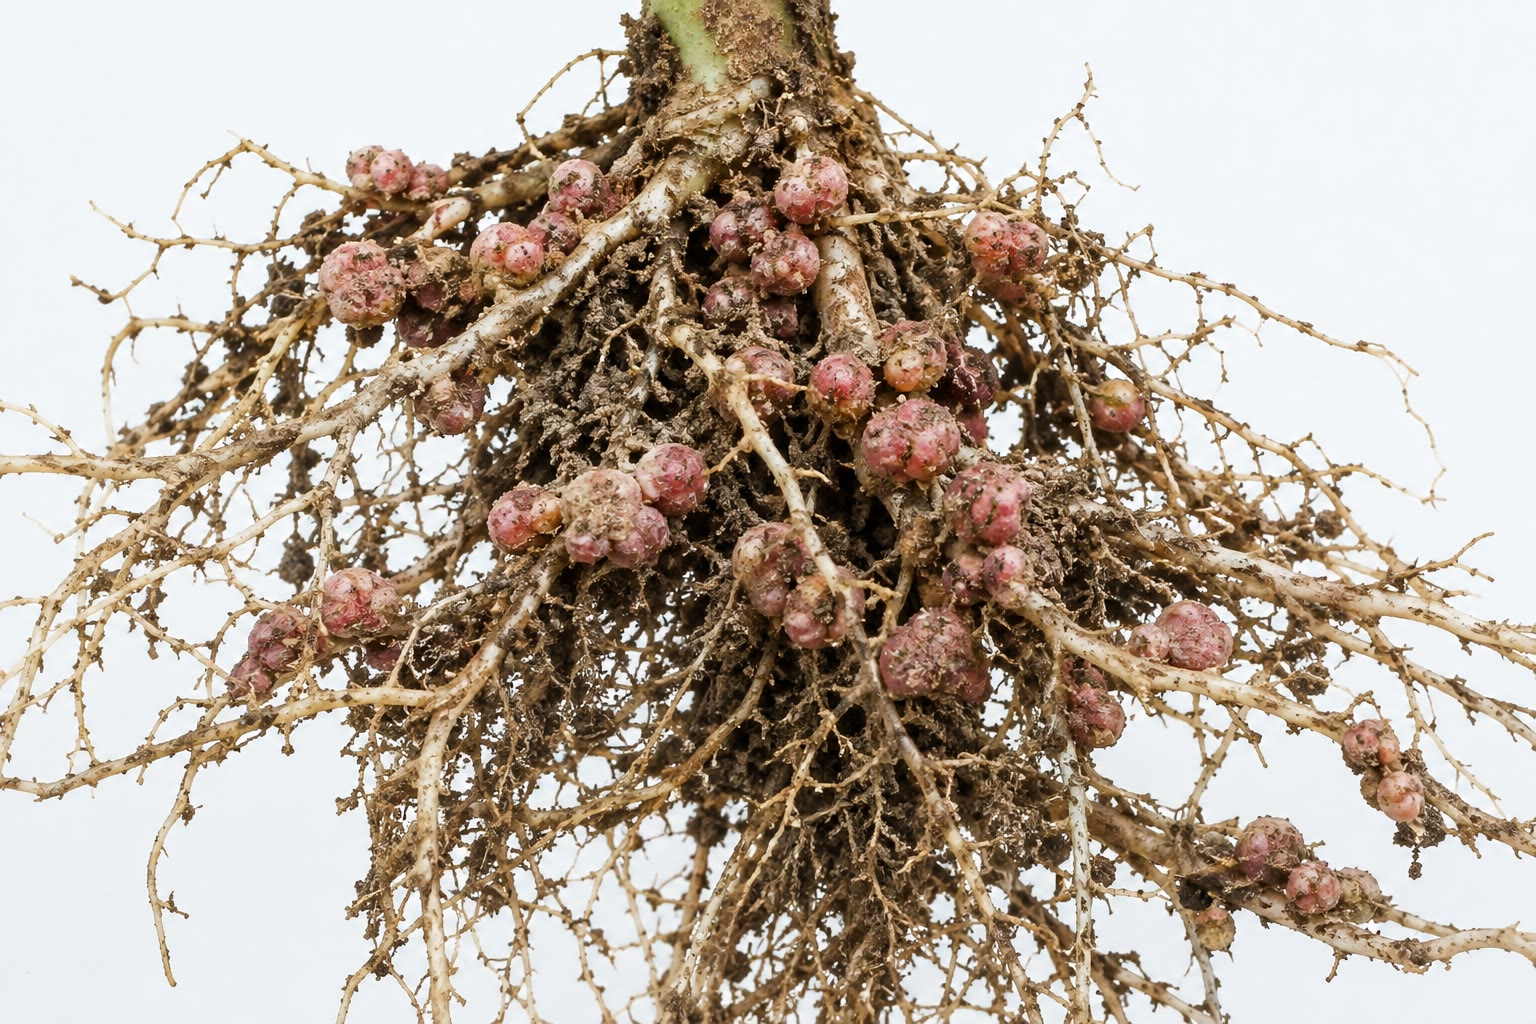
\includegraphics[width=0.46\linewidth]{images/book5/ai/b5-14-root-nodules.jpg}\hspace{0.04\linewidth}
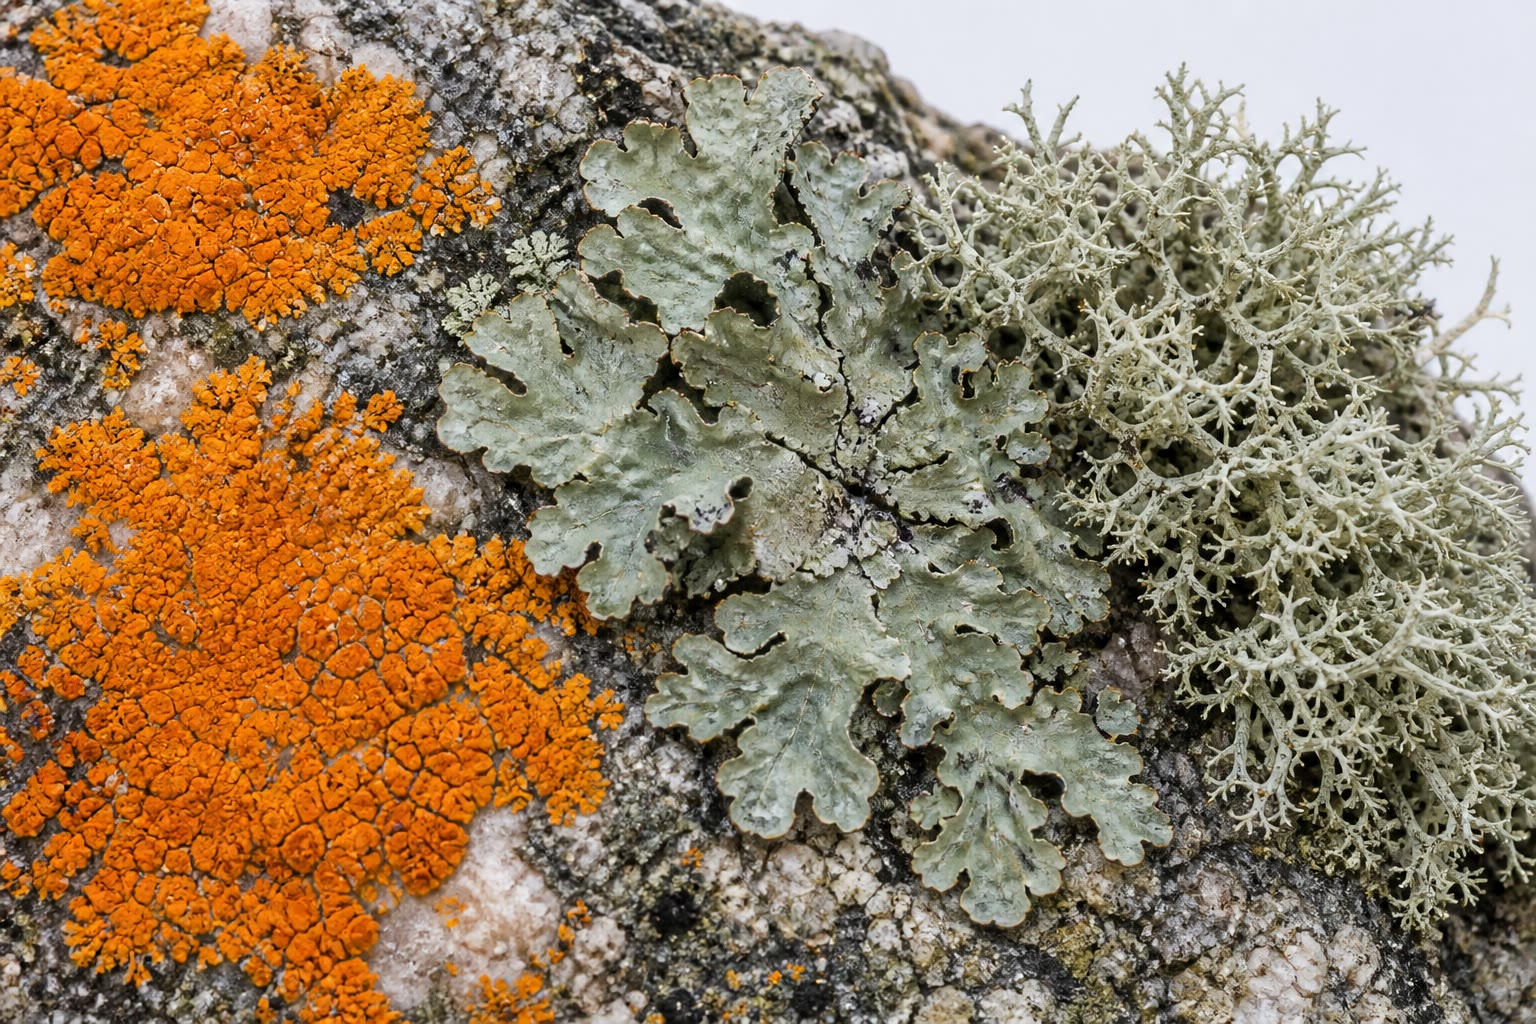
\includegraphics[width=0.46\linewidth]{images/book5/ai/b5-14-lichen.jpg}

{\small 左：豆科植物的结瘤根，每个粉红色\omterm{def:b3:microbiomes:nodule}{根瘤}都是
由糖供养的类菌体构成的固氮工厂。右：岩石上的地衣，
——每一个都是真菌容纳光合藻类或蓝细菌的\omterm{def:b3:microbiomes:symbiosis}{共生}体，
共同定植于单独任何一方都无法占据的表面。}
\end{omfigure}

\section{海洋及其他地方的伙伴关系}

\begin{definition}[珊瑚与藻类]\label{def:b3:microbiomes:coral}
\index{珊瑚共生}\index{虫黄藻}\index{珊瑚白化}
造礁珊瑚的肠壁内衬细胞中寄居着甲藻（\emph{Symbiodiniaceae}，
即\emph{虫黄藻}），每平方厘米一百万个或更多。
藻类在动物组织内进行光合作用，
利用动物排出的废物 CO$_{2}$、氨和磷酸盐，
并将多达\qty{90}{\%}的固定碳，以甘油、糖类和氨基酸的形式
回输给宿主，供养珊瑚及构建珊瑚礁的钙化作用；
珊瑚则反过来控制藻类的氮供应，进而决定其生长。
这一伙伴关系只在很窄的温度范围内成立：
当水温高出夏季最高值约一至两度，
并持续数周时，藻类的光合作用受损，
它们向宿主细胞释放活性氧，珊瑚便将其排出，
即\emph{白化}——白色骨骼透过半透明的动物体显露出来。
白化的珊瑚会挨饿；
若水温在数周内降温，它便能恢复，否则即死亡。
自 1980 年以来，白化的频率已升至原来的五倍，
这正是变暖使珊瑚礁消失的机制。
\end{definition}

\begin{example}[制造栖息地的共生关系]\label{ex:b3:microbiomes:habitats}
\emph{地衣}是一种真菌，内部容纳一种绿藻或蓝细菌，
真菌提供结构、保水功能以及从岩石中溶解的矿物质，
光合\omterm{def:b3:microbiomes:symbiosis}{共生}体提供糖类（若为蓝细菌，还提供氮）；
地衣覆盖约\qty{8}{\%}的陆地表面，定植于裸露岩石，
并开始将其转化为土壤。深海热液喷口的管虫
\emph{Riftia}成体没有口腔或肠道；
它在营养体中容纳硫化物氧化细菌，并借助
能同时结合两者的血红蛋白，向其输送硫化物和氧气，
在黑暗中全靠化学能，每年生长超过一米。白蚁借助
肠道内由原生生物和细菌组成的群落消化木材；反刍动物则消化草料，
依靠瘤胃消化，瘤胃大小相当于一只浴缸，其中细菌、古菌与
真菌将纤维素发酵为脂肪酸和甲烷；牛以脂肪酸和
微生物自身的躯体为食。在每种情形中，
一种代谢能力——光合作用、固氮、
硫化物氧化、纤维素消化——是宿主谱系从未进化出的，
却在一步之内借助伙伴关系获得。
\end{example}

\begin{omfigure}
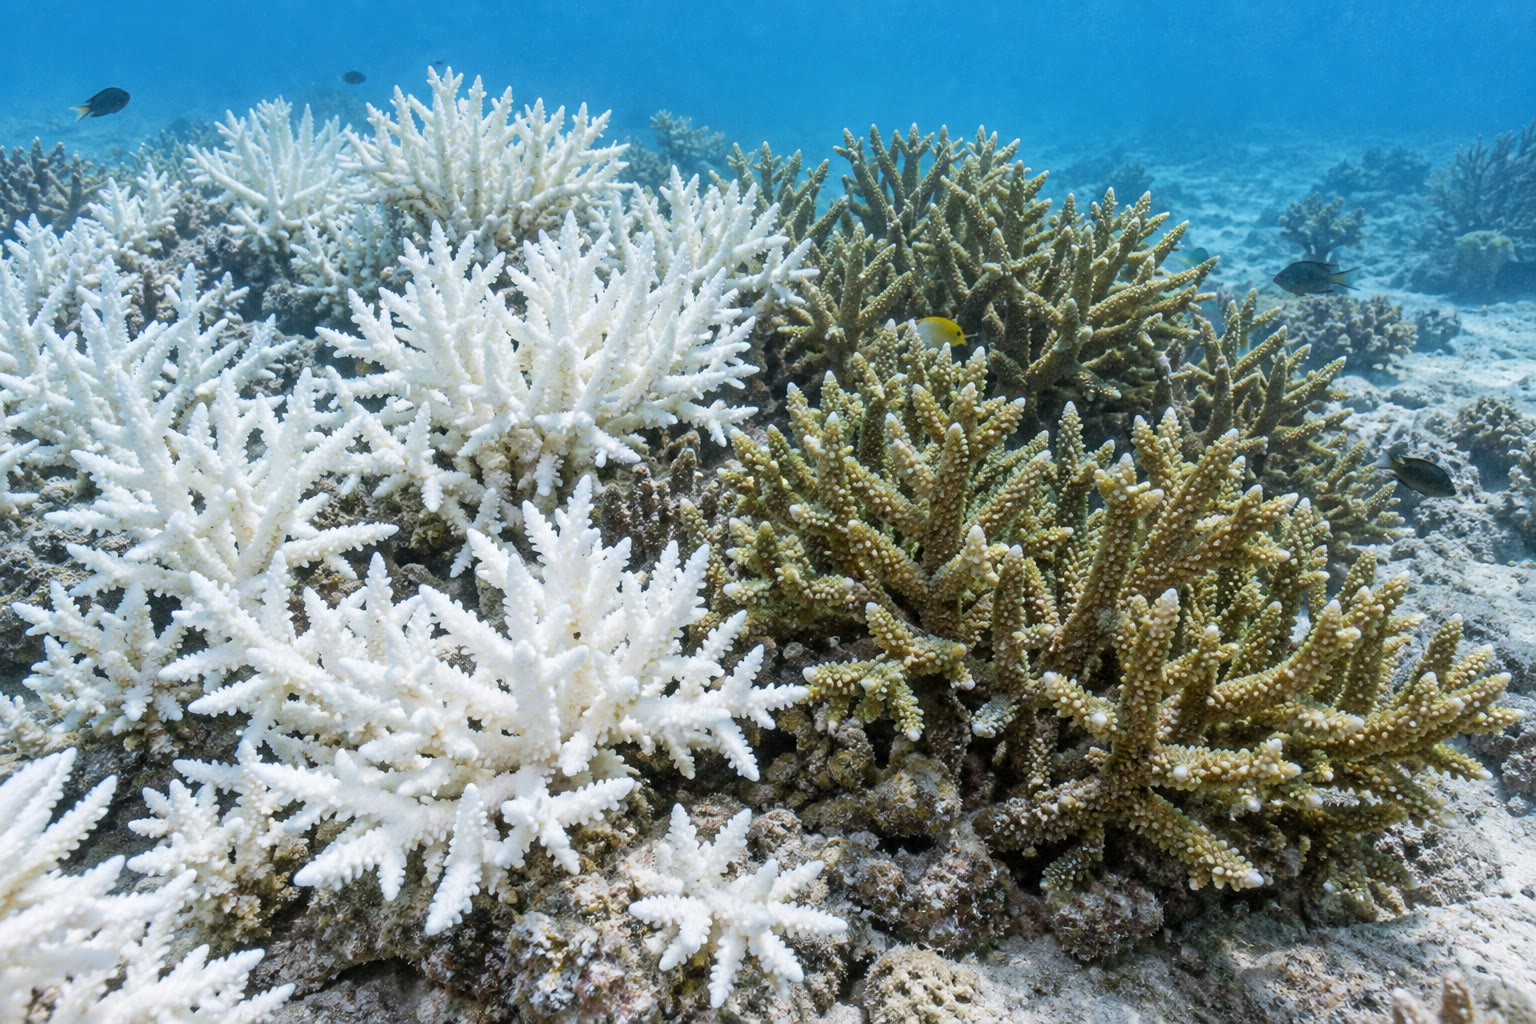
\includegraphics[width=0.56\linewidth]{images/book5/ai/b5-14-coral-bleaching.jpg}

{\small 半白化的珊瑚礁：白色群体已排出了
藻类，原因是水温过高持续数周；棕色群体仍保有其藻类。
白色珊瑚仍然存活但正在挨饿，尚有数周时间可以重新定植。}
\end{omfigure}

\begin{omfigure}
\begin{tikzpicture}[every node/.style={font=\scriptsize}, >=stealth]
  % coral cell with alga
  \draw[very thick, omDef, fill=omDef!8] (0,0) ellipse (3.2 and 2.0); \node[above] at (0,2.05) {珊瑚细胞（胃皮层）};
  \draw[thick, omMeth!70!black, fill=omMeth!30] (-0.4,-0.1) circle (1.05); \node[align=center] at (-0.4,-0.1) {藻类 \\（虫黄藻）};
  % exchanges
  \draw[->, thick, omMeth!70!black] (0.5,0.4) -- (1.9,0.9) node[right, align=left] {甘油、糖类、氨基酸：\\最多\qty{90}{\%}的固定碳};
  \draw[<-, thick, omThm] (0.5,-0.5) -- (1.9,-1.0) node[right, align=left] {CO$_2$、NH$_3$、磷酸盐 \\（动物的废物）};
  \draw[<-, thick, omProp] (-1.3,0.3) -- (-2.6,1.0) node[left, align=right] {透过 \\组织的光};
  \node[below, align=center] at (1.5,-2.1) {胁迫：水温高，持续数周 $\to$ 光合作用受损，\\活性氧 $\to$ 藻类被排出 $\to$ 白化};
  % thermometer-like bar on the right
  \begin{scope}[xshift=7.6cm, yshift=-1.6cm]
    \draw[thick] (0,0) rectangle (0.5,3.2);
    \fill[omDef!40] (0,0) rectangle (0.5,2.0); \fill[omProp!60] (0,2.0) rectangle (0.5,2.6); \fill[omThm!60] (0,2.6) rectangle (0.5,3.2);
    \node[right] at (0.6,1.0) {正常范围}; \node[right] at (0.6,2.3) {$+\qty{1}{\celsius}$：胁迫}; \node[right, align=left] at (0.6,2.9) {$+\qty{2}{\celsius}$ 持续数周：\\白化};
    \node[below, align=center] at (0.25,-0.1) {夏季海水 \\温度};
  \end{scope}
\end{tikzpicture}

{\small 珊瑚–藻类之间的交换：藻类利用
动物的废物和透过组织的光固定碳，并将其中大部分
以食物形式返还；温度持续小幅升高即会破坏这一伙伴关系。}
\end{omfigure}

\section{从伙伴到细胞器}

\begin{proposition}[基因组缩减与通往细胞器之路]\label{prop:b3:microbiomes:reduction}
\index{基因组缩减}\index{内共生基因转移}
通过卵遗传的内\omterm{def:b3:microbiomes:symbiosis}{共生}体生活在一个由少数细胞组成的种群中，
这些细胞从不与外界重组。对它的选择很弱
（\cref{ch:b3:molecular-evolution}：小种群通过遗传漂变固定略有害的
突变），产物由宿主提供的基因损坏时
不会被察觉，丢失的基因永远无法重新获得。因此基因组
逐代缩小——\emph{Buchnera}
缩至\qty{640}{kb}，一些昆虫\omterm{def:b3:microbiomes:symbiosis}{共生}体缩至\qty{140}{kb}、仅含数百个基因，
线粒体缩至\qty{16}{kb}，人类线粒体中仅有十三种蛋白质——
而宿主的细胞核获得了\omterm{def:b3:microbiomes:symbiosis}{共生}体基因的拷贝，
借助\emph{\omterm{prop:b3:microbiomes:reduction}{内共生基因转移}}，其产物
需借靶向序列被运回。当宿主制造\omterm{def:b3:microbiomes:symbiosis}{共生}体的大部分蛋白质、控制其分裂，
并且自身离不开它时，
\omterm{def:b3:microbiomes:symbiosis}{共生}体便成为细胞器。线粒体与质体
分别在二十亿年前和十亿年前走过这条道路，
（本科一年级分册）；\emph{Paulinella}的色素体是第三者，
走过此路，已历时约一亿年。
\end{proposition}

\begin{remark}[再论个体]\label{rem:b3:microbiomes:individual}
动物或植物是以基因组为中心的群落，其代谢功能的大部分，
以及发育和免疫的很大一部分，
都依赖于它未在自身 DNA 中继承的伙伴。实际后果已然显现：
\omterm{def:b3:microbiomes:symbiosis}{微生物组}可作为药物（粪便移植），
可作为药物的作用靶点（\omterm{def:b3:bacteriology:antibiotics}{抗生素}的附带损害、膳食纤维作为处方），
可作为诊断手段，并作为一条途径——
通过工程化\omterm{def:b3:microbiomes:symbiosis}{共生}体和携带\emph{Wolbachia}的蚊子，
以改变野生种群的生物学特性。
理论上的一点是：自然选择作用于伙伴关系，
而最强的伙伴关系，
正是一方的命运同时决定另一方的那些伙伴关系。
\end{remark}

\section{练习}

\begin{exercise}[$\star$]\label{exo:b3:microbiomes:1}
定义\omterm{def:b3:microbiomes:symbiosis}{互利共生}、\omterm{def:b3:microbiomes:symbiosis}{偏利共生}和寄生，并各举一例（取自本章）。
为什么同一对物种能在
这些类别之间转换？
\end{exercise}

\begin{exercise}[$\star$]\label{exo:b3:microbiomes:2}
计算下列丰度所对应群落的 $H$、$e^{H}$、$D$ 和 $1/D$：
丰度分别为 $0.5$、$0.3$、$0.1$、$0.05$、$0.05$。
\end{exercise}

\begin{exercise}[$\star$]\label{exo:b3:microbiomes:3}
比较 16S 扩增子调查与鸟枪法\omterm{met:b3:microbiomes:16s}{宏基因组学}：二者各报告什么，
以及各自无法告诉你什么？
\end{exercise}

\begin{exercise}[$\star$]\label{exo:b3:microbiomes:4}
列出\omterm{def:b3:microbiomes:gut}{肠道微生物组}为其宿主提供的四项服务，以及
其失调后随之而来的一种疾病。
\end{exercise}

\begin{exercise}[$\star\star$]\label{exo:b3:microbiomes:5}
一份样本含 $N = 20$ 条读段，各物种的读段数为 $N_{i} = 10, 6, 3, 1$。
利用定理计算 $E[S_{n}]$（取 $n = 5$），以及\omterm{thm:b3:microbiomes:rarefaction}{古德覆盖度}。
\end{exercise}

\begin{exercise}[$\star\star$]\label{exo:b3:microbiomes:6}
结肠含内容物 \qty{400}{g}，每克内容物中含 $10^{11}$ 个
细菌；每个细菌重 \qty{1}{pg}，其基因组含 \num{4000} 个
基因；一个人的肠道中有 $1000$ 个物种。估算
\omterm{def:b3:microbiomes:symbiosis}{微生物组}的质量及其携带的不同基因数，并
与人类基因组的 \num{20000} 个基因相比。
\end{exercise}

\begin{exercise}[$\star\star$]\label{exo:b3:microbiomes:7}
解释\omterm{def:b3:microbiomes:nodule}{根瘤}的氧悖论，以及\omterm{def:b3:microbiomes:nodule}{豆血红蛋白}与
扩散屏障如何解决这一悖论。为什么\omterm{def:b3:microbiomes:nodule}{根瘤}呈粉红色，
而绿色\omterm{def:b3:microbiomes:nodule}{根瘤}意味着什么？
\end{exercise}

\begin{exercise}[$\star\star$]\label{exo:b3:microbiomes:8}
一个豆科植物突变体缺失\omterm{def:b3:microbiomes:mycorrhiza}{共同共生途径}中的钙振荡成分，
请预测其结瘤和\omterm{def:b3:microbiomes:mycorrhiza}{菌根}化情况，
并解释这一结果对两种\omterm{def:b3:microbiomes:symbiosis}{共生}关系的演化说明了什么。
\end{exercise}

\begin{exercise}[$\star\star$]\label{exo:b3:microbiomes:9}
描述基尔斯的\omterm{prop:b3:microbiomes:sanctions}{制裁}实验，并预测若植物无法区分固氮\omterm{def:b3:microbiomes:nodule}{根瘤}与非固氮\omterm{def:b3:microbiomes:nodule}{根瘤}，
会出现怎样的结果。
\end{exercise}

\begin{exercise}[$\star\star\star$]\label{exo:b3:microbiomes:10}
证明\omterm{def:b3:microbiomes:diversity}{稀疏化}定理中的 $E[S_{n}]$ 是 $n$ 的递增函数，
且 $S$ 为其在 $n = N$ 处的取值；并证明对满足 $N_{i} \ll N$ 与 $n \ll N$ 的物种，
其被观测到的概率约为
$1 - (1 - n/N)^{N_{i}}$。
\end{exercise}

\begin{exercise}[$\star\star\star$]\label{exo:b3:microbiomes:11}
\emph{Wolbachia} 只经卵传递。解释为何对其的选择有利于雌性宿主，
描述胞质不亲和，
并说明为何即使
感染带来较小代价，感染株仍能扩散。
\end{exercise}

\begin{exercise}[$\star\star\star$]\label{exo:b3:microbiomes:12}
利用\cref{prop:b3:microbiomes:reduction}，解释为何垂直传递的内\omterm{def:b3:microbiomes:symbiosis}{共生}体
的基因组会缩小，而自由生活的近缘种则不会，
哪些基因最先丢失、哪些最后丢失，以及
什么会逆转这一趋势。
\end{exercise}

\section{问题：肠道普查}

\begin{problem}[{周末问题——以细胞、基因和热量计量的肠道微生物组，
测量并稀疏化其多样性，
平衡豆科植物的氮收支与糖分，核算珊瑚礁的碳，
末尾为微生物组获取的热量、测序样本的覆盖度，
以及豆田为固氮付出的
糖分}]
\label{pb:b3:microbiomes:1}
数据：结肠内容物 \qty{400}{g}，每克含 $10^{11}$ 个细菌，单个细胞
质量 \qty{1}{pg}；$1000$ 个物种，每个含 \num{4000} 个基因，
任意两个物种之间共享 \qty{30}{\%} 的基因。饮食：每天 \qty{30}{g} 膳食纤维，
经发酵生成\omterm{def:b3:microbiomes:gut}{短链脂肪酸}，产率为每克 \qty{10}{mmol}，
各价值 \qty{0.9}{kJ}；饮食能量为 \qty{9000}{kJ}。测序样本：
$N = 2000$ 条读段，$S = 180$ 个物种，$f_{1} = 60$ 个单例；前三个物种的
丰度分别为 $0.30$、$0.20$、$0.10$，其余物种均匀分布。
一茬豆类作物每公顷每季固定 \qty{150}{kg} 氮，并
为每克所固定的氮付出 \qty{8}{g} 糖；其光合作用每季每公顷产糖
\qty{12}{t}。\omterm{def:b3:microbiomes:nodule}{固氮酶}：$16$ 个
ATP 固定一个 N$_{2}$。一块珊瑚含 $10^{6}$ 个藻类（每 cm$^{2}$），每个藻类每天固定 \qty{20}{pg}
碳，其中 \qty{90}{\%} 转给宿主；珊瑚组织
每 cm$^{2}$ 每天呼吸消耗 \qty{15}{\micro g} 碳。

\medskip
\noindent\textbf{第一部分——细胞与基因。}
\begin{enumerate}
  \item 结肠中有多少细菌？它们的总重量是多少？
  \item 这些 DNA 相当于多少个细菌基因组？其总量与
        $3\times 10^{13}$ 个人类细胞中的 DNA 相比如何（每个细胞
        \qty{6.4}{pg}）？
  \item 估算肠道中不同细菌基因的数目，
        计入 \qty{30}{\%} 的重叠（每个物种计其未共享的
        \qty{70}{\%} 基因，再加一组共享基因集）。与
        \num{20000} 相比。
  \item 膳食纤维每天产生多少毫摩尔\omterm{def:b3:microbiomes:gut}{短链脂肪酸}，
        折合能量多少千焦，
        占饮食的比例为多少？
  \item 无菌小鼠需要多 \qty{30}{\%} 的食物。第 4 问中的脂肪酸
        贡献是否足以解释这一点？
        还可能是什么原因？
  \item 细菌在结肠中约每天分裂一次，内容物
        以相同速率排出。这意味着何种稳态，
        以及一个疗程的\omterm{def:b3:bacteriology:antibiotics}{抗生素}
        杀死 \qty{99.9}{\%} 的细胞时，群落会发生什么变化？
\end{enumerate}

\medskip
\noindent\textbf{第二部分——多样性。}
\begin{enumerate}[resume]
  \item 计算 $177$ 个次要物种各自的相对丰度，
        再求\omterm{def:b3:microbiomes:diversity}{香农指数} $H$ 与 $e^{H}$。
  \item 计算\omterm{def:b3:microbiomes:diversity}{辛普森指数} $D$ 与 $1/D$。为何 $1/D$ 小于
        $e^{H}$？
  \item 样本的\omterm{thm:b3:microbiomes:rarefaction}{古德覆盖度}为多少，每千条读段中有多少属于
        未观测到的物种？
  \item 从同一肠道取得的第二个样本含 \num{10000} 条读段，
        得到 $260$ 个物种。利用稀疏定理解释这为何不构成矛盾，
        并说明
        比较两者之前应做什么。
  \item 在该定理中，$N_{i} = 1$ 的物种出现在
        $n = 1000$ 的子样本中的概率是多少，其中 $N =
        2000$？$N_{i} = 5$ 时又是多少？
  \item 使用\omterm{def:b3:bacteriology:antibiotics}{抗生素}后，同一肠道出现 $60$ 个物种，$H = 2.0$，
        有一个物种的丰度为 $0.5$。计算 $e^{H}$ 与 $D$，
        并用文字描述该群落。
\end{enumerate}

\medskip
\noindent\textbf{第三部分——\omterm{def:b3:microbiomes:nodule}{根瘤}的账目。}
\begin{enumerate}[resume]
  \item 作物每公顷为其
        \qty{150}{kg} 氮支付多少糖，
        这占其光合作用的比例为多少？
  \item \qty{150}{kg} 氮相当于多少摩尔 N$_{2}$，
        \omterm{def:b3:microbiomes:nodule}{固氮酶}为此消耗多少摩尔 ATP？
  \item 按每分解一个葡萄糖可产生 $30$ 个 ATP 计算，
        这些 ATP 相当于多少千克葡萄糖？与所支付的糖相比，
        其余部分用于什么？
  \item 工业合成氨每千克氮约需 \qty{35}{MJ}。
        取每克糖 \qty{16}{kJ}，比较作物
        固氮与工厂合成氨的能量成本。
  \item 一个不固氮的\omterm{def:b3:microbiomes:nodule}{根瘤菌}进入\omterm{def:b3:microbiomes:nodule}{根瘤}。若植株将其氧气减半作为惩罚，
        其繁殖量减半，
        若作假者起始占 \qty{10}{\%}，固氮者正常繁殖，则下一季
        \omterm{def:b3:microbiomes:nodule}{根瘤菌}中作假者占多少？
        （仅计一轮。）
  \item 若无惩罚，省去固氮成本的作假者繁殖量高出 \qty{20}{\%}，
        从相同起点出发，十个季节后作假者占多少？
        这一比较说明了什么？
\end{enumerate}

\medskip
\noindent\textbf{第四部分——珊瑚礁的账目。}
\begin{enumerate}[resume]
  \item 每平方厘米藻类每天固定多少碳，
        其中有多少进入珊瑚？
  \item 与珊瑚的呼吸作用相比，盈余为多少，
        这些盈余用于什么？
  \item 白化后，\qty{95}{\%} 的藻类消失。重新计算所供应的碳，
        珊瑚以每 cm$^{2}$ 含 \qty{300}{\micro g} 碳的储备，
        能维持多久？
  \item 胁迫常以“度热周”衡量，
        即季节中每周超出夏季最高温度的部分之和。
        八周 $+\qty{1}{\celsius}$ 与四周 $+\qty{2}{\celsius}$ 均得 $8$；
        白化通常在 $4$ 左右开始。
        两种情形中哪一种更严重？
        为何该指标仍可能有效？
  \item 珊瑚可同时容纳多种耐热极限不同的藻类，
        试提出珊瑚礁可能如何适应，以及何种因素限制这种适应。
  \item 一个面积为 \qty{1}{km^2} 的活珊瑚礁表面，
        其藻类每天及每年固定多少吨碳？
  \item 总结：\omterm{def:b3:microbiomes:symbiosis}{微生物组}所供应的饮食比例
        （第 4 题）、测序样本的覆盖度
        （第 9 题），以及豆类作物为其氮所支付的
        光合作用比例（第 13 题）。
\end{enumerate}
\end{problem}
